%
% abstrakt.tex
%
% (c) 2018 Prof Dr Andreas Müller, Hochschule Rapperswil
%
\documentclass[tikz]{standalone}
\usepackage{times}
\usepackage{amsmath}
\usepackage{txfonts}
\usepackage[utf8]{inputenc}
\usepackage{graphics}
\usetikzlibrary{arrows,intersections,math}
\usepackage{ifthen}
\begin{document}

\newboolean{showgrid}
\setboolean{showgrid}{false}
\def\breite{7}
\def\hoehe{4}

\begin{tikzpicture}[>=latex,thick]

% Povray Bild
\node at (0,0) {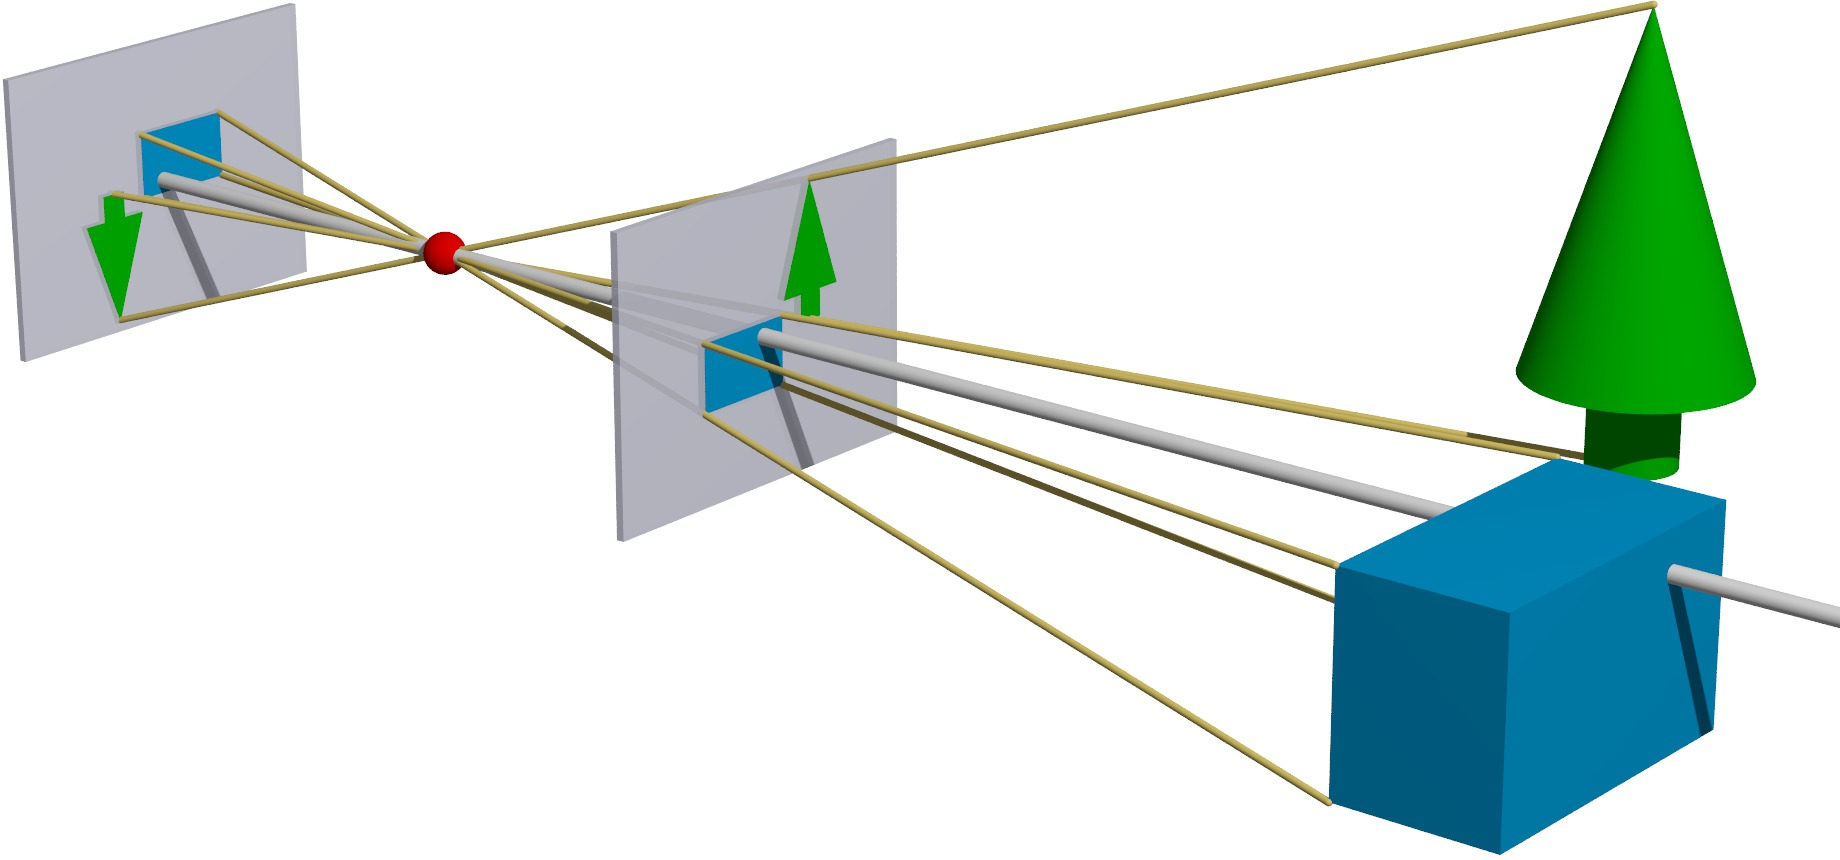
\includegraphics[width=14cm]{abstrakt.jpg}};

% Beschriftungen
\node at (-3.6,1.5) [above] {$C$};
\node at (5.6,3.2) [above right] {$P$};
\node at (-0.8,1.9) [above] {$B$};
\node at (-6.1,0.8) [below] {$B'$};
\node at (-2,-0.5) {$\beta$};
\node at (-6.5,2.4) {$\beta'$};
\node at (-2.6,1.4) {$f$};
\node at (-4.5,1.3) {$f$};
\node at (6.7,-1.1) {$z$};
\node at (0,1.1) {$y$};
\node at (-1.2,1.8) [above left] {$x$};

% Gitter
\ifthenelse{\boolean{showgrid}}{
\draw[step=0.1,line width=0.1pt] (-\breite,-\hoehe) grid (\breite, \hoehe);
\draw[step=0.5,line width=0.4pt] (-\breite,-\hoehe) grid (\breite, \hoehe);
\draw                            (-\breite,-\hoehe) grid (\breite, \hoehe);
\fill (0,0) circle[radius=0.05];
}{}

\end{tikzpicture}

\end{document}

